\begin{frame}
    \frametitle{Interfaces}
    \begin{itemize}
        \item {\large Web Site:}
        \begin{itemize}
            \item Should all the user to do any task in the least amount of 
            clicks
            \item Should look visually appealign, with lack of ``clutter''
        \end{itemize}
        \item {\large Android Device:}
        \begin{itemize}
            \item Follow same UI and visual requirements as the website
            \item Will allow the user to log in via a wireless technology
        \end{itemize}
    \end{itemize}
\end{frame}

\subsection{Website}
\begin{frame}
    \frametitle{Website}
    \begin{itemize}
        \item Django/Python, HTML, CSS, Javascript
        \item PostgreSQL
        \item Administrative functions
    \end{itemize}
\end{frame}

\subsection{Android Device}
\begin{frame}
    \frametitle{Android Device}
    \begin{itemize}
        \item {\large Nexus 7}
        \begin{itemize}
            \item App will be build in the Android version of Java and XML
            \item Device will be attached to the DRINC machine
        \end{itemize}
    \end{itemize}
\end{frame}

\begin{frame}
    \frametitle{Android Mock-up}
    \begin{figure}[htb]
        \centering
        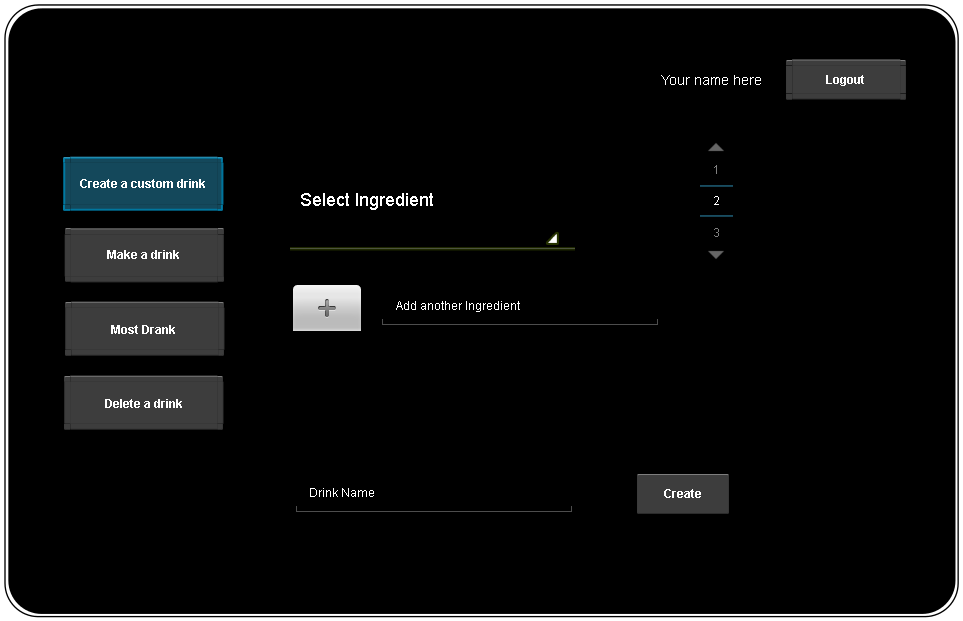
\includegraphics[width=0.8\textwidth]{../Mock-ups/Android_CreateDrink.png}
        \caption{Example of creating a drink on the Android device}
        \label{fig:CreateDrinkAndroid}
    \end{figure}
\end{frame}
\begin{frame}
    \frametitle{Android Mock-up}
    \begin{figure}[htb]
        \centering
        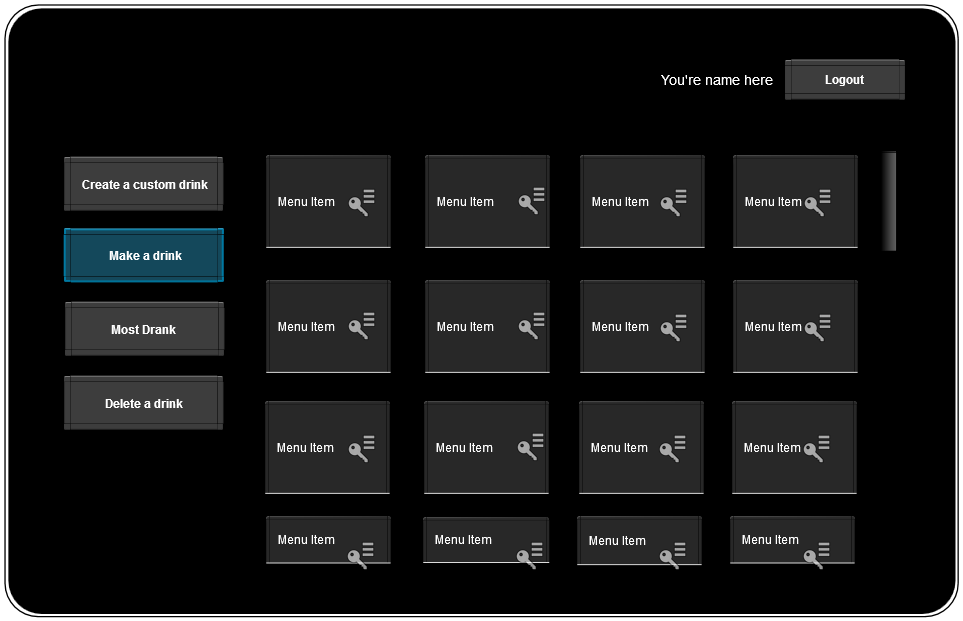
\includegraphics[width=0.8\textwidth]{../Mock-ups/Android_SelectDrink.png}
        \caption{Example of selecting a drink on the Android device}
        \label{fig:SelectingDrinkAndroid}
    \end{figure}
\end{frame}
